\chapter{Materials and Methods}
\section{\Nsm\space strains used in this work}
\begin{table}[h]
\begin{center}
\begin{tabular}{>{\centering}m{4.4cm}m{6.4cm}>{\centering}m{3.1cm}}
\toprule
\textbf{Name} & \centering \textbf{Description} & \textbf{Source}
\tabularnewline
\midrule
MC58 & Wild-Type Strain & \citet{McGuinness1990}
\tabularnewline\noalign{\smallskip}\hline\noalign{\smallskip}
$\Delta$norB::spc$^\textrm{r}$\nomenclature{spc$^\textrm{r}$}{Spectinomycin resistance} & Wild-Type with insertion of spectinomycin resistance cassette into \textit{norB} gene & \citet{Heurlier2008}
\tabularnewline\noalign{\smallskip}\hline\noalign{\smallskip}
$\Delta$nsrR::spc$^\textrm{r}$ & Wild-Type with insertion of spectinomycin resistance cassette into \textit{nsrR} gene & \citet{Rock2007}
\tabularnewline\noalign{\smallskip}\hline\noalign{\smallskip}
$\Delta$norB::spc$^\textrm{r}$-$\Delta$nsrR::tet$^\textrm{r}$\nomenclature{tet$^\textrm{r}$}{Tetracyclin resistance} & Wild-Type with insertion of spectinomycin resistance cassette into \textit{norB} and insertion of tetracyclin resistance cassette into \textit{nsrR} genes & \citet{Heurlier2008}
\tabularnewline\noalign{\smallskip}\hline\noalign{\smallskip}
$\Delta$aniA::spc$^\textrm{r}$-$\Delta$nsrR::tet$^\textrm{r}$ & Wild-Type with insertion of spectinomycin resistance cassette into \textit{aniA} and insertion of tetracyclin resistance cassette into \textit{nsrR} genes & \citet{Heurlier2008}
\tabularnewline
\bottomrule
\end{tabular} 
\end{center}
\caption{Bacterial strains and sources
\label{tab:bacterial-strains}}
\end{table}

\section{Culturing \Nsm}
\subsection{Growth of \Nsm}
\Nm\space strains were grown on plates on Columbia Agar Base (CAB)\nomenclature{CAB}{Columbia Agar Base} with defibrinated horse blood, and in liquid culture in Muller-Hinton Broth (MHB)\nomenclature{MHB}{Muller-Hinton Broth}.

Plates were prepared by adding horse blood to a final concentration of 5\% to molten agar, and poured into plastic petri dishes. After streaking with \Nm\space the plates were incubated at 37\textdegree C in a 5\% carbon dioxide/air mixture.

Aerobic liquid cultures were grown in 10ml MHB with 1\% NaHCO$_\textrm{3}$ in plastic sterilin tubes, and incubated at 37\textdegree C at 200rpm\nomenclature{rpm}{Revolutions Per Minute}. Microaerobic cultures were suspended in 20ml MHB, 1\% NaHCO$_\textrm{3}$ in plastic sterilin tubes, incubated at 37\textdegree C at 100rpm.

\subsection{Preparation of Antibiotic Selective Media}
Liquid stock solutions of required antibiotics were either added directly to liquid culture, or, if growing on plates, to the molten agar when also adding horse blood. The final concentrations of antibiotics are given in Table \ref{tab:antibiotic-concs}.

\begin{table}[here]
\begin{center}
\begin{tabular}{cc}
\toprule
\textbf{Antibiotic} & \textbf{Final concentration ($\mu$g/ml)} \\
\midrule
Spectinomycin & 50 \\
Tetracyclin & 2.5 \\
Chloramphenicol & 50 \\
\bottomrule
\end{tabular} 
\end{center}
\caption{Final antibiotic concentrations
\label{tab:antibiotic-concs}}
\end{table}

\subsection{Preparation of Frozen Bacterial Stocks}
Bacteria were grown in liquid culture until late log phase prior to harvesting. Liquid cultures were then centrifuged at 4000g for 15 minutes, and the pellet was then resuspended in a 25\% glycerol, 25\% water and 50\% MHB, all of which had been autoclaved beforehand. The bacterial stocks were then frozen at $-80$\textdegree C.

\subsection{Streaking Plates for OD to CFU Ratio Calculation}
Bacterial cultures were grown overnight and then transferred into aerobic liquid culture and samples taken throughout the day to obtain a range of different optical densities. The optical density was recorded at 600nm, and each sample was serially diluted to the following levels: $10^{-5}$, $10^{-6}$ and $10^{-7}$. 100$\mu$l of each of these dilutions was plated on a fresh blood agar plate and left to grow overnight. The following morning the number of colonies on each plate was counted and used to create a standard curve for Optical Density\nomenclature{OD}{Optical Density} to Colony Forming Units\nomenclature{CFU}{Colony Forming Units}.

\section{Measuring Oxygen Concentration}
Oxygen concentration in respiring cultures was measured using a Clark electrode \cite{Clark1953} from Rank Brothers, Cambridge, UK. This electrode has a silver anode and a platinum cathode using a saturated potassium chloride solution as electrolyte. The electrode is set at the bottom of a ~7ml reaction chamber separated from its contents by a thin teflon membrane. This membrane is permeable to dissolved oxygen, and is reduced by the electrode producing a measurable electrical current. The reaction chamber is maintained at 37\textdegree C by an attached waterbath.
When performing experiments, 5ml of culture is added to the reaction chamber, which is stirred by use of a magnetic flea, and the chamber covered with a plastic stopper. The stopper has a number of holes through which the NO probe, or hamilton syringe can be inserted. Data is collected by attaching the electrode to an external data logger (Pico ADC20, Pico Technology).
\subsection{Calibration of Oxygen Electrode}
Calibration of the oxygen electrode assumes that anaerobic water will not produce any measurable current at the electrode. Oxygen saturated water contains 210$\mu$M Oxygen (ref needed). 5ml of ultrapure water was added to the electrode chamber, and then aerated to saturation by use of a pasteur pipette. The maximum value recorded by the data logger then corresponds to a concentration of 210$\mu$M Oxygen, with the relationship between mV as recorded against concentration being linear.

\section{Measuring Nitric Oxide Concentration}
Nitric Oxide concentration was measured using a Nitric Oxide probe (ISO-NOP, World Precision Intruments) connected to a Nitric Oxide Meter (ISO-NO mkII, World Precision Instruments). This is also a Clark type electrode, contained within a steel sleeve with a semi-permeable membrane separating the working electrode from the system being measured\cite{Liu2005,Bedioui2003,Serpe2007}. The NO probe is inserted through one of the holes in the plastic lid of the reaction chamber of the oxygen electrode assembly. The tip of the electrode should be immersed in the culture, with care being taken not to trap any air bubbles on the surface of the probe. The sensor is also attached to the same data logger as above. In this way both Oxygen and Nitric Oxide concentrations can be measured in parallel.
\subsection{Calibration of Nitric Oxide Electrode}
Calibration of the nitric oxide electrode 

\section{Measuring Nitrite Concentration (Griess Assay)}
\cite{DonaldNicholas1957}
\subsection*{Chemicals}
\begin{itemize}
 \item 50ml 1\% w/v Sulfanilamide in 1M HCl
 \item 50ml 0.02\% w/v NED\nomenclature{NED}{\textit{N}-1-napthylethylenediamine dihydrochloride} in 1M HCl
\end{itemize}


\section{Nitric Oxide Production}
Similar to the setup described by \cite{Aga2008}.
\begin{figure}
 \centering
 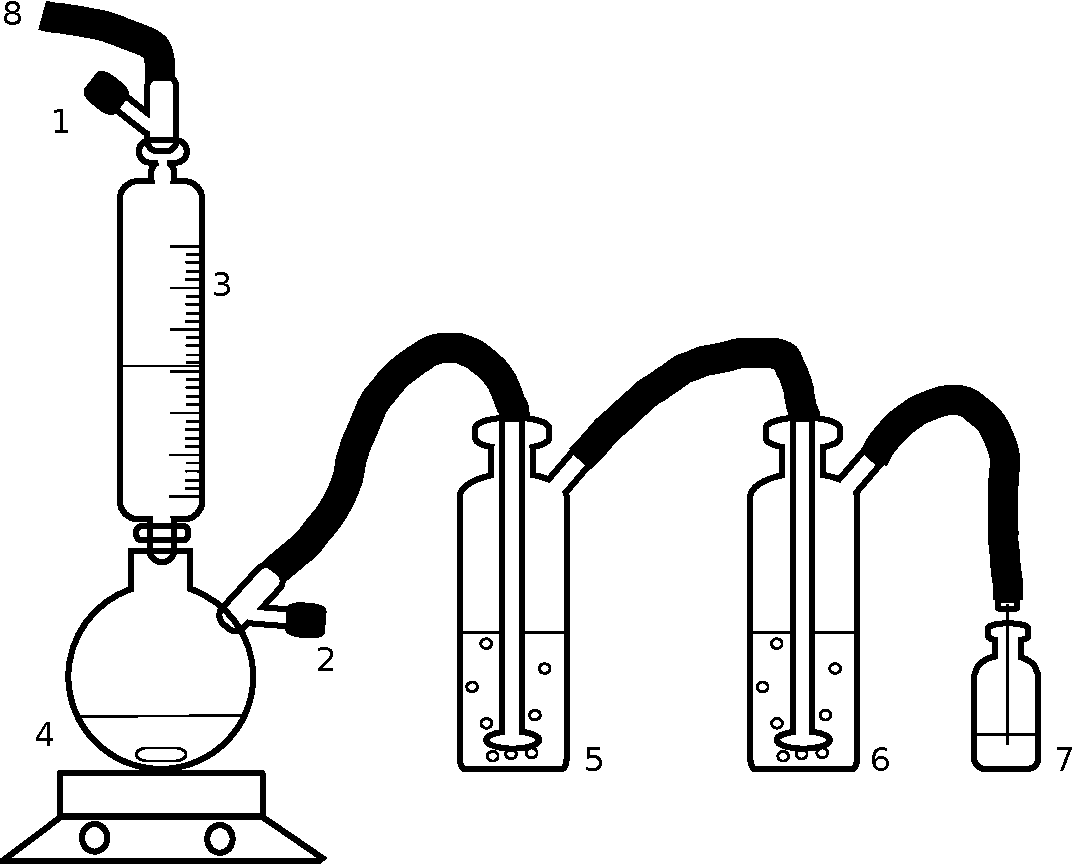
\includegraphics[width=14cm]{./02-materialsmethods/data/drawing.pdf}
 % drawing.pdf: 515x415 pixel, 72dpi, 18.17x14.64 cm, bb=0 0 515 415
 \caption{\footnotesize NO making apparatus. 1,2 - N$_{\textrm{2}}$ release valve. 3 - 50ml 4M H$_{\textrm{2}}$SO$_{\textrm{4}}$. 4 - 200ml 2M NaNO$_{\textrm{2}}$ stirring. 5 - 1M NaOH $\frac{2}{3}$ full. 6,7 - dH$_{\textrm{2}}$O $\frac{2}{3}$ full. 8 - To N$_{\textrm{2}}$ gas bottle.}
\end{figure}
\subsection*{Chemicals}
\begin{itemize}
 \item 200ml NaNO$_{\textrm{2}}$ @ 2M - 27.6g in 200ml dH$_{\textrm{2}}$O
 \item 50ml H$_{\textrm{2}}$SO$_{\textrm{4}}$ @ 4M - 11ml in 39ml dH$_{\textrm{2}}$O
 \item 200ml NaOH @ 1M - 8g in 200ml dH$_{\textrm{2}}$O
\end{itemize}

\subsection*{Procedure}
\begin{itemize}
 \item Set up system and sparge with N$_{\textrm{2}}$ gas for 15 minutes. Sparge 4M H$_{\textrm{2}}$SO$_{\textrm{4}}$ separately.
 \item Shut valve to N$_{\textrm{2}}$ hose (blue valve 1).
 \item Keep blue valve 2 open at all times.
 \item When sparged, add 25ml of 4M H$_{\textrm{2}}$SO$_{\textrm{4}}$ to 2M NaNO$_{\textrm{2}}$ and allow brown gas to bubble through to saturated solution vessel.
 \item Leave for at least 15 minutes allow 2M solution to cool.
 \item Remove needle and close sealing valve on saturated solution vessel.
 \item Clean up - allow 1-2 hours to allow reaction to finish. Sparge with N$_{\textrm{2}}$ to get rid of residual NO gas. Disassemble, wash in dH$_{\textrm{2}}$O and dry in oven.
\end{itemize}

\section{Solving Ordinary Differential Equations}
An ordinary differential equation solver was written in Java utilising a 6th-order Runge-Kutta algorithm with adaptive step-size as described by \citet{WilliamH.Press1992}